% Project:     IMS project
% @file        doc/simulation_study.tex
% @date        29.11.2023
% 
% @brief Simulation study file
%
% @author Adam Ližičiar <xlizic00@stud.fit.vutbr.cz>

\documentclass[a4paper, 11pt]{article}

\usepackage[slovak]{babel}
\usepackage[utf8]{inputenc}
\usepackage[left=2cm, top=3cm, text={17cm, 24cm}]{geometry}
\usepackage{times}
\usepackage{verbatim}
\usepackage{enumitem}
\usepackage[slovak, boxed]{algorithm2e}
\usepackage{listings}
\usepackage{color}
\usepackage{graphicx}
\usepackage{tabularx}
\usepackage[unicode]{hyperref}
\hypersetup{
    colorlinks=true,
    linkcolor=black,
    urlcolor=blue, 
    citecolor=blue
}
\definecolor{mygreen}{rgb}{0,0.6,0}
\definecolor{mygray}{rgb}{0.5,0.5,0.5}
\definecolor{mymauve}{rgb}{0.58,0,0.82}
\lstset{
  backgroundcolor=\color{white},
  basicstyle=\footnotesize,
  breaklines=true,
  captionpos=b,
  commentstyle=\color{mygreen},
  escapeinside={\%*}{*)},
  keywordstyle=\color{blue},
  stringstyle=\color{mymauve},
  tabsize=4
}


\begin{document}

	%%%%% Titulná stránka %%%%%
	\begin{titlepage}
		\begin{center}
			
\includegraphics[width=0.77\linewidth]{resources/logo_FIT.pdf} \\

			\vspace{\stretch{0.382}}

			\scalebox{2}{\Huge{Simulačná štúdia}} \\
			\LARGE{Transport tovaru spoločnosťou DALITRANS, s.r.o.} \\
			\vspace{\stretch{0.618}}
		\end{center}

		\begin{minipage}[b]{0.4 \textwidth}
			\raggedright
			{\Large \today}
		\end{minipage}
		\hfill
		\begin{minipage}[b]{0.6 \textwidth}
			\raggedleft
			\Large
			Adam Ližičiar (xlizic00)\\
		\end{minipage}		
	\end{titlepage}

	%%%%% Obsah %%%%%
	\pagenumbering{roman}
	\setcounter{page}{1}
	\tableofcontents
	\clearpage

	\pagenumbering{arabic}
	\setcounter{page}{1}
	
	%%%%% Úvod %%%%%
	\section{Úvod}
	Práca sa~zaoberá rozvozom tovaru spoločnosti DALITRANS, s.r.o.,
    konkrétne pomerom využiteľnosti kamiónov na počet jázd za mesiac.
    Vďaka tomuto modelu a~simulačnému experimentu je~možné pozorovať
    efektívnosť aktuálneho systému a~nájsť spôsoby na~zefektívnenie
    tohoto systému. Spoločnosť je~zameraná na~vnútroštátnu i~zahraničnú prepravu,
    preto tento model opisuje obdobie jedného mesiaca. Táto doba
    je~aktuálne používaná i v~rámci firmy pre~sprehľadnenie počtu jázd,
    účtovných uzávierok a~v~neposlednom rade kvôli štatistickým
    potrebám. V~modeli je~vždy používaný 30-dňový formát mesiaca.\newline
    V~reálnom systéme je~náročné zisťovať ekonomické rozdiely, pretože
    systém obsahuje veľké množstvo entít a~faktorov, ktoré s~nimi súvisia.
    Výsledkom preto budú faktory na~zefektívnenie využívania aktuálneho systému,
    ktoré by bez modelu nebolo možné zistiť.

    \subsection{Zdroje faktov}
	Informácie o~tranzitnej spoločnosti boli získané z~jej oficiálnej
    webstránky\cite{DaliTrans}, štatistických údajov
    spoločnosti\cite{DaliTransFinstat} a~od
    majiteľa firmy Dalibora Janegu.
    Pri práci bola taktiež použitá prezentácia z predmetu
    Modelování a simulace\cite{IMSprezentácia}
    a~online webová stránka o knižnici \cite{SIMLIB}.\newline
    Autorom tejto simulačnej štúdie je Adam Ližičiar.\newline

    %%%%% Fakty %%%%%
    \newpage
	\section{Fakty}
    Všetky fakty, ktoré nemajú pri~sebe odkaz na~zdroj, boli zistené priamo
    od~majiteľa firmy.\newline
    \newline
    K~aktuálnemu dátumu je~v spoločnosti
    267~tranzitných vozidiel (väčšina Renault Trucks
    520 T-High). Tieto vozidlá majú kombinovanú spotrebu pri~naloženom prívese
    34~litrov na~100 kilometrov a~pri~prázdnom prívese 22~litrov
    na~100 kilometrov.\cite{RenualtTrucks}\newline
    Jazdy sú~už~vopred tak naplánované, že~po~dokončení jazdy je~šofér
    vyslaný na~ďaľšiu jazdu, ku~ktorej sa~dostane
    za~64~minút ±~23~minút.
    Dovolenky alebo ochorenia zamestnancov nie~je~potrebné riešiť
    z~dôvodu dostatočného počtu voľných zamestnancov a~taktiež
    podrobnému naplánovaniu jázd, kedy sa každý vodič vráti po~približne
    5~dňoch v~práci na~depo (kamión prevezme ďalší zamestnanec). Počet
    voľných zamestnancov nie~je~potrebné riešiť z~dôvodu, že~ich 
    je~dostatočný počet a~v~ojedinelom prípade, kedy by nikto zo~zamestnancov
    nebol dostupný, sú~volaní externí šoféri. Každý mesiac
    je~vykonaných 5083 jázd  ± 256 jázd. Pravdepodobnosť poruchy
    kamióna je 2,3~\%. Jej následná oprava trvá 2 hodiny 
    (niektoré poruchy vyžadujú omnoho dlhší čas, avšak vo~veľkej väčšine
    sa~jedná o~rýchloodstrániteľné poruchy).\newline
    Prechod k~prvému zákazníkovi na miesto nakladania trvá priemerne 
    64~minút ±~23~minút (vzdialenosť 85~km ±~28~km). Následne prebehne naloženie (46~minút ±~21~minút).
    Po naložení sa vodič vyberie na jazdu, ktorá trvá 14 hodín ± 10 hodín
    (v~čase sú~započítané aj povinné pauzy podľa štandartov Európskej
    únie). Dĺžka trasy je 605~km  ± 421~km.
    Po~vyložení tovaru (28 minút ± 14 minút) si~šofér spraví 6~hodinovú prestávku
    a~pokračuje k~ďalšiemu zákazníkovi (64~minút ±~23~minút). Pri~prevoze je~vždy v~prívese
    tovar iba od~jedného zákazníka.\cite{DaliTrans}\newline


    %%%%% Koncepcia a spôsob riešenia %%%%%
	\newpage
    \section{Koncepcia a~spôsob riešenia}
	V modeli sú~zahrnuté všetký potrebné a~dôležité fakty z~kapitoli
    č.~2. Počet jázd je~už~vopred známy (väčšinou sú~jazdy vo~firme objednávané
    s predstihom 3 mesiacov), preto generátor prichádzajúcich jázd nie je~potrebný.
    Firma vždy prijme približne 5083 jázd  ± 256 jázd na jeden mesiac.
    Proces prijímania taktiež nezohráva žiadnu rolu, pretože ponúk 
    na~prevoz je vždy dostatočný a jazdy, ktoré sa nezmestia alebo
    sú~nevhodné pre firmu sú odmietnuté. Taktiež približne 70~percent
    jázd tvoria pravidelne opakujúce sa zásobovacie jazdy.\newline
    Za~zmienku stojí aj rozdelenie modelu do mesačných blokov, v~ktorom
    každý mesiac pozostáva vždy z 30 dní.
    
    \subsection{Prevod riešenia do Petriho siete}
    Petriho sieť (príloha \ref{subsection:petrinet}) sa skladá z 4 hlavných častí.
    Prvou časťou je~riadenie aktivity modelu, ktorá má za~úlohu sledovať
    stav počtu jázd a~taktiež mesačného časovača a v~prípade vyčerpania všetkých
    naplánovaných jázd alebo ukončenia časovača ukončí model.
    Druhou hlavnou časťou je~model kamióna zahrňujúci prechod k~zákazníkovi,
    naloženie, jazdu, vyloženie, pauzu a~možnú poruchu kamióna.
    Treťou časťou je~časovač mesiaca, ktorý na~začiatku modelu začne
    počítať čas a dohliada, či už nebolo prekročených 30~dní.
    V prípade, ak by táto situácia nastala, bude program ukončený
    a~niekoľko jázd (1 a~viac) bude nedokončených.
    Poslednou štvrtou časťou je~úspešné ukončenie v~prípade vyčerpania
    všetkých jázd pod dobu 1 mesiaca od~začatia jázd. 

    \subsection{Implementácia riešenia}
    Model je~vytvorený v~programovacom jazyku C++. Na~simuláciu je~použitá knižnica
    SIMLIB, ktorá obsahuje všetky časti potrebné k~implementácií modelu.

    \subsubsection{Hlavný súbor}
    Súbor \texttt{main.c} obsahuje základnú funkciu \texttt{int main(int argc, char *argv[])},
    v~ktorej prebieha iterácia počtu vopred určených simulácií (prednastavený na~3
    v~premennej \texttt{NUM\_OF\_SIMULATION\_ATTEMPS} v~\texttt{src/Libraries/main.hpp}).
    Okrem tejto funkcie obsahuje hlavný súbor ešte funkcie na~výpis začiatku a~konca 
    simulácie na štandartný chybový výstup.

    \begin{algorithm}[ht]
		\SetKw{Break}{break}
		výpis začiatku simulácie\;
		\For{\(i = 1; i \leq \texttt{NUM\_OF\_SIMULATION\_ATTEMPS}; i++\)}
		{
			vypíš začiatok konkrétnej simulácie\;
            vytvor a aktivuj konkrétnu simuláciu\;
            vypíš výsledok konkrétnej simulácie\;
		}
        vypíš koniec simulátora\;
		\caption{Preudokód \texttt{main.cpp}}
		\label{algorithm:mainfile}
	\end{algorithm}

    \subsubsection{Použité triedy}
    \paragraph{Arguments}
    Trieda slúži na~parsovanie argumentov. Má~povinné argumenty \texttt{-t/--trucks},
    ktorá reprezentuje počet kamiónov a~\texttt{-j/--journeys}, ktorá reprenzetuje
    počet jážd. Taktiež je~možné využiť volitelný argument \texttt{-h/--help}
    na~výpis informácií o~argumentov.
    
    \paragraph{ModelActivity}
    Riadi aktivitu jednotlivých simulácií. Obsahuje vo~funkcii
    \texttt{void ModelActivity::Behavior()} cyklus ukázaný v \textbf{Algoritmus \ref{algorithm:simulacia}}.
    \begin{algorithm}[ht]
		\SetKw{Break}{break}

		výpis začiatku simulácie\;
		\While{naplánované jazdy sú~nenulové}
		{
			zobratie voľného kamióna (ak je k~dispozící, ak nie je, tak čaká na~voľný kamión)\;
			\eIf{nie sú už~žiadne jazdy}
			{
				uvoľnenie kamióna\;
				\Break\;
			}
			{
				odpočítanie počtu jázd o~1\;
				aktivácia modelu kamióna\;
			}
		}
		čakanie na nulový počet jázd a na~vrátenie sa~všetkých kamiónov\;
		ukončenie\;

		\caption{Pseudokód jednej simulácie}
		\label{algorithm:simulacia}
	\end{algorithm}
    
    \paragraph{MonthTimer}
    Časovač, ktorý dohliada, či nebol prekročený mesiac v modelovom čase od spustenia programu.

    \paragraph{Truck}
    Obsahuje implementáciu kamióna od cesty k zákazníkovi, cez nakladanie, jazdu s nákladom,
    vyloženie, pauzu a možnú poruchu kamióna.

    \paragraph{UniformGenerator}
    Generuje náhodné čísla s normálovým rozložením. Generátor vygeneruje
    pri každom pokuse iné číslo, čo zlepšuje výsledok s ohľadom na náhodnosť
    javov. Pri každom pokuse bolo použitých 10 vzorkov, ktoré boli spriemerované.

    \subsubsection{Knižnice}
    Na simuláciu v programe je použitá knižnica SIMLIB\cite{SIMLIB}.\newline
    Taktiež sú využité štandartné knižnice ako \texttt{iostream},
    \texttt{stdlib.h} ako aj \texttt{getops.h} na prácu s argumentami a
    \texttt{random}, \texttt{chrono} a \texttt{time.h} na generovanie
    náhodných čísel.

    \subsection{Spúštanie simulačného modulu}
    Pre spustenie je najskôr potrebný jeho preklad a následne spustenie buď
    pomocou preddefinovaných parametrov alebo vlastných parametrov:
\begin{lstlisting}
// moznost s preddefinovanymi parametrami
make
make run
    
// moznost s vlastnymi parametrami
make
./bin/simulation -t/--trucks X -j/--journeys Y
\end{lstlisting}   

    %%%%% Testovanie a experimenty %%%%%
    \newpage
	\section{Testovanie a experimenty}
	Cieľom experimentov je v prvom rade overiť validitu modelu a~následne
    hľadať možné vylepšenia aktuálneho systému.
    Vo~všetkých experimentoch boli najskôr vložené vstupné hodnoty, 
    s~ktorými simulácia vykonala svoju činnosť a~vrátila výsledky. Tieto
    výsledky boli spriemerované a~vypísané do~tejto simulačnej štúdie.

    \subsection{Experimenty}
    \subsubsection{Overenie validity}
    Vstupnými hodnotami sú hodnoty získané z faktov, t.j. 267 kamiónov
    a 5083 jázd. Po vykonaní experimentu je výsledok, že model je valídny,
    pretože všetkých 10 vykonaných experimentoch bolo ukončených úspešne
    s dostatočnou rezervou.
    \begin{table}[ht]
		\centering
		\begin{tabular}{|r|r|r|r|}
			\hline
			Počet kamiónov & Počet jázd & Ubehnutý čas/celkový čas [m] & \textbf{Správnosť modelu} \\ \hline
			267 & 5124 & 30 053/43 200 &\textbf{100\%} \\ \hline
		\end{tabular}

		\caption{Experiment: Overenie validity}
		\label{table:1}
	\end{table}

    \subsubsection{Maximálny počet jázd}
    Vstupná hodnota počtu trás bola postupne zvyšovaná, pokiaľ nenastalo prekročenie
    počtu jázd, ktoré sú schopné kamióny za mesiac previesť. Experiment bol vykonaný
    10 krát pre každý pokus s jedinečnými vstupnými údajmi a hodnoty spriemerované.\newline
    Z výsledkov plynie, že maximálny počet jázd na 267 kamiónov je 7942, po tomto čísle
    úspešnosť postupne klesá k 0 percentám.
    \begin{table}[ht]
		\centering
		\begin{tabular}{|r|r|r|r|}
			\hline
			Počet kamiónov & Počet jázd & Ubehnutý čas/celkový čas [m] & \textbf{Správnosť modelu} \\ \hline
			267 & 5495 & 28 692/43 200 &\textbf{100\%} \\ \hline
            267 & 6012 & 31 100/43 200 &\textbf{100\%} \\ \hline
            267 & 6541 & 33 802/43 200 &\textbf{100\%} \\ \hline
            267 & 7942 & 41 087/43 200 &\textbf{100\%} \\ \hline
            267 & 8208 & 42 138/43 200 &\textbf{80\%} \\ \hline
            267 & 8516 & 43 200+/43 200 &\textbf{30\%} \\ \hline
            267 & 8687 & 43 200+/43 200 &\textbf{0\%} \\ \hline
		\end{tabular}

		\caption{Experiment: Maximálny počet jázd}
		\label{table:2}
	\end{table}

    \subsubsection{Minimálny počet kamiónov na~aktuálny počet jázd}
    V tomto  experimente sa mení počet kamiónov a zachováva sa stály počet
    jázd. Experiment bol vykonaný
    10 krát pre každý pokus s jedinečnými vstupnými údajmi a hodnoty boli spriemerované.\newline
    Z výsledkov plynie, že minimálny počet kamiónov pre zachovanie
    100 percentnej úspešnosti a priemerného počtu jázd za mesiac je 170.
    \begin{table}[ht]
		\centering
		\begin{tabular}{|r|r|r|r|}
			\hline
			Počet kamiónov & Počet jázd & Ubehnutý čas/celkový čas [m] & \textbf{Správnosť modelu} \\ \hline
			267 & 5124 & 28 692/43 200 &\textbf{100\%} \\ \hline
            240 & 5080 & 29 568/43 200 &\textbf{100\%} \\ \hline
            200 & 5043 & 35 126/43 200 &\textbf{100\%} \\ \hline
            180 & 5052 & 38 709/43 200 &\textbf{100\%} \\ \hline
            170 & 5109 & 40 976/43 200 &\textbf{100\%} \\ \hline
            160 & 5095 & 43 200+/43 200 &\textbf{70\%} \\ \hline  
		\end{tabular}

		\caption{Minimálny počet kamiónov na~aktuálny počet jázd}
		\label{table:3}
	\end{table}

    \subsubsection{Počet jázd po zrušení 6 hodinovej prestávky po jazde a pri zachovaní počtu kamiónov}
    Počet kamiónov zostáva stály, zvyšuje sa počet jázd a je zrušená 6 hodinová
    prestávka po jazde.\newline
    Z uvedeného vyplýva, že po zrušení 6 hodinovej prestávky by bolo možné
    spraviť s tým istým počtom kamiónov viac než dvojnásobný počet jázd
    pri 100 úspešnosti. 
    
    \begin{table}[ht]
		\centering
		\begin{tabular}{|r|r|r|r|}
			\hline
			Počet kamiónov & Počet jázd & Ubehnutý čas/celkový čas [m] & \textbf{Správnosť modelu} \\ \hline
			267 & 5124 & 19 612/43 200 &\textbf{100\%} \\ \hline
            267 & 5499 & 20 967/43 200 &\textbf{100\%} \\ \hline
            267 & 6521 & 24 906/43 200 &\textbf{100\%} \\ \hline
            267 & 7508 & 28 498/43 200 &\textbf{100\%} \\ \hline
            267 & 8436 & 32 054/43 200 &\textbf{100\%} \\ \hline
            267 & 9454 & 35 685/43 200 &\textbf{100\%} \\ \hline
            267 & 10 505 & 39 460/43 200 &\textbf{100\%} \\ \hline
            267 & 11 497 & 43 144/43 200 &\textbf{100\%} \\ \hline
            267 & 12 042 & 43 200+/43 200 &\textbf{60\%} \\ \hline
		\end{tabular}

		\caption{Počet jázd po zrušení 6 hodinovej prestávky po jazde a pri zachovaní počtu kamiónov}
		\label{table:4}
	\end{table}


    %%%%% Záver %%%%%
    \clearpage
	\section{Záver}
	Zo záveru vyplýva, že je možné so zachovaním 100\% úspešnosti
    zvýšiť počet jázd na 7 942 za mesiac. V prípade zachovania počtu jázd
    stačí používať o 97 kamiónov menej (z 267 na 170). Ak by došlo
    k zrušeniu vodičskej 6 hodinovej prestávky po jazde, bolo by možné
    za mesiac vykonať viac než dvojnásobný počet jázd.\newline
    Z experimentov vyplýva jednoznačné doporučenie, aby spoločnosť
    DaliTrans zvýšila počet jázd za mesiac alebo znížila počet svojich
    kamiónov.\newline
    Výsledky týchto experimentov sú správne, pretože bola najskôr
    overená validita modelu a pri každom experimente bolo vykonaných min. 70 pokusov.
    Spolu bolo aj s validáciou modelu vykonaných 231 experimetov, ktoré boli
    spriemerované do jednotlivých výsledkov. 

 
	%%%%% Literatúra %%%%%
    \newpage
	\section{Literatúra}
	\bibliographystyle{bibliography/czechiso}
    \renewcommand{\refname}{}
	\bibliography{bibliography/simulation_study}

	%%%%% Prílohy %%%%%
    \clearpage
	\appendix
	\section{Prílohy}
    \subsection{Petriho sieť}
	\label{subsection:petrinet}
	\begin{figure}[!ht]
		\centering
		\vspace{1cm}
		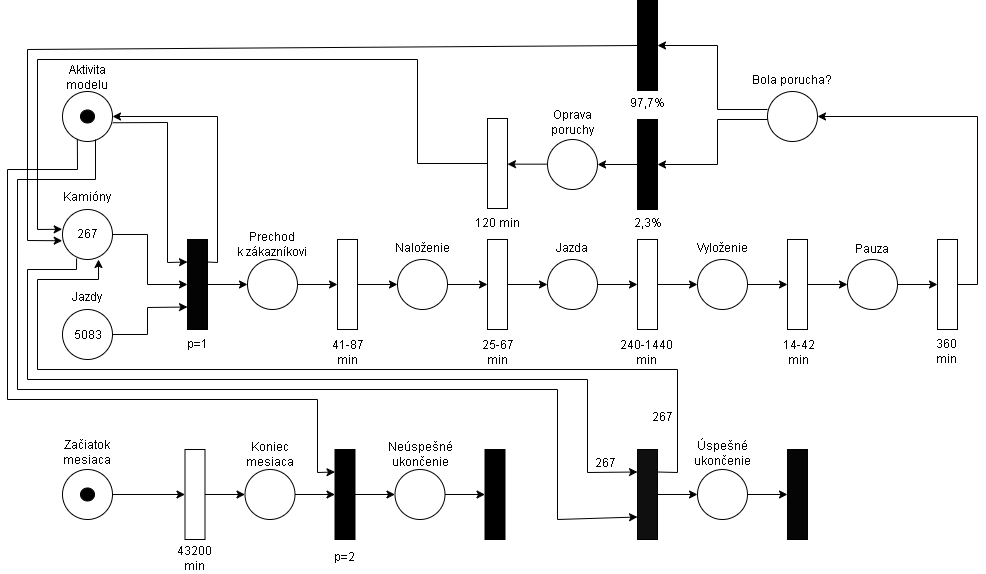
\includegraphics[width=0.95\linewidth]{resources/petri_net.png}
		\caption{Petriho sieť modelu}
		\label{figure:petri_net}
	\end{figure}

\end{document}
